\documentclass[border=2pt]{standalone}
\usepackage{tikz}
\usetikzlibrary{arrows.meta,positioning,calc}
\usepackage{amsmath}
\begin{document}
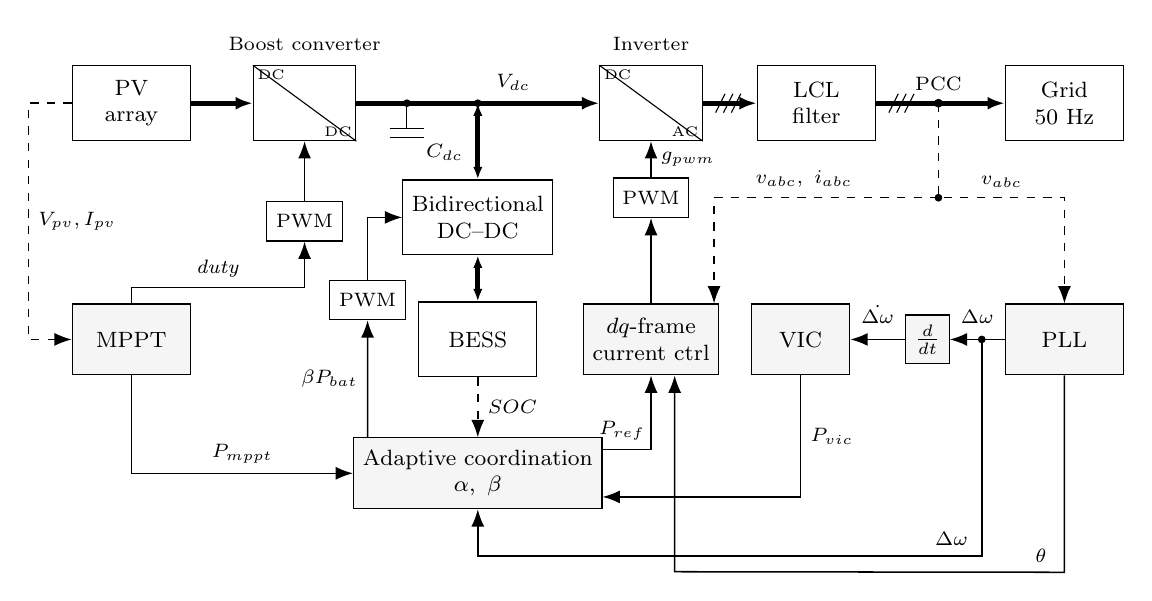
\begin{tikzpicture}[
    font=\footnotesize,
    >={Latex[length=2.2mm]},
    blk/.style={rectangle, draw, minimum width=1.5cm, minimum height=0.95cm, align=center},
    conv/.style={rectangle, draw, minimum width=1.3cm, minimum height=0.95cm},
    pwmb/.style={rectangle, draw, minimum width=0.7cm, minimum height=0.5cm, align=center},
    cblk/.style={rectangle, draw, fill=gray!8, minimum width=1.5cm, minimum height=0.9cm, align=center},
    pw/.style={->, line width=1.7pt},
    sig/.style={->, line width=0.55pt},
    ms/.style={->, line width=0.55pt, dashed}
]
% ---- power chain ----
\node[blk] (pv) at (0,0) {PV\\array};
\node[conv] (boost) at (2.2,0) {};
\draw (boost.north west) -- (boost.south east);
\node[anchor=north west, inner sep=1.5pt] at (boost.north west) {\tiny DC};
\node[anchor=south east, inner sep=1.5pt] at (boost.south east) {\tiny DC};
\node[anchor=south] at (2.2,0.55) {\scriptsize Boost converter};
\node[conv] (inv) at (6.6,0) {};
\draw (inv.north west) -- (inv.south east);
\node[anchor=north west, inner sep=1.5pt] at (inv.north west) {\tiny DC};
\node[anchor=south east, inner sep=1.5pt] at (inv.south east) {\tiny AC};
\node[anchor=south] at (6.6,0.55) {\scriptsize Inverter};
\node[blk] (fil) at (8.7,0) {LCL\\filter};
\node[blk] (grid) at (11.85,0) {Grid\\$50$ Hz};
\draw[pw] (pv) -- (boost);
\draw[pw] (boost) -- (inv);
\draw[pw] (inv) -- (fil);
\draw[pw] (fil) -- (grid);
% kapasitor DC-link pada bus DC
\fill (3.5,0) circle (1.4pt);
\draw (3.5,0) -- (3.5,-0.32);
\draw (3.28,-0.32) -- (3.72,-0.32);
\draw (3.28,-0.44) -- (3.72,-0.44);
\node[anchor=west] at (3.62,-0.62) {\scriptsize $C_{dc}$};
\node[anchor=south] at (4.85,0.04) {\scriptsize $V_{dc}$};
% tanda saluran tiga fase
\foreach \x in {7.42,7.52,7.62} \draw ($(\x,-0.12)$) -- ($(\x+0.12,0.12)$);
\foreach \x in {9.62,9.72,9.82} \draw ($(\x,-0.12)$) -- ($(\x+0.12,0.12)$);
\coordinate (pcc) at (10.25,0);
\fill (pcc) circle (1.6pt);
\node[above=1pt] at (pcc) {\scriptsize PCC};
% ---- PWM blocks ----
\node[pwmb] (pwm2) at (2.2,-1.5) {\scriptsize PWM};
\draw[sig] (pwm2.north) -- (boost.south);
\node[pwmb] (spwm) at (6.6,-1.2) {\scriptsize PWM};
\draw[sig] (spwm.north) -- (inv.south) node[midway, right] {\scriptsize $g_{pwm}$};
\node[pwmb] (pwmb3) at (3.00,-2.5) {\scriptsize PWM};
% ---- BESS on the DC side ----
\node[blk] (bidir) at (4.4,-1.45) {Bidirectional\\DC--DC};
\node[blk] (bess)  at (4.4,-3.0) {BESS};
\fill (4.4,0) circle (1.4pt);
\draw[pw, {Latex[length=1.6mm]}-{Latex[length=1.6mm]}] (4.4,0) -- (bidir.north);
\draw[pw, {Latex[length=1.6mm]}-{Latex[length=1.6mm]}] (bidir) -- (bess);
\draw[sig] (pwmb3.north) -- (3.00,-1.45) -- (bidir.west);
% ---- control layer ----
\node[cblk] (mppt) at (0,-3.0)  {MPPT};
\node[cblk] (ctrl) at (6.6,-3.0) {$dq$-frame\\current ctrl};
\node[cblk, minimum width=1.25cm] (vic)  at (8.50,-3.0) {VIC};
\node[cblk] (pll)  at (11.85,-3.0) {PLL};
\node[cblk, minimum width=3.0cm] (coord) at (4.4,-4.7) {Adaptive coordination\\$\alpha,\ \beta$};
% pengukuran PV -> MPPT
\draw[ms] (pv.west) -- ++(-0.55,0) node[midway, above] {} |- (mppt.west) node[pos=0.25, right] {\scriptsize $V_{pv}, I_{pv}$};
% MPPT -> duty boost
\draw[sig] (mppt.north) -- ++(0,0.20) -| (pwm2.south) node[pos=0.25, above] {\scriptsize \textit{duty}};
% MPPT -> koordinasi
\draw[sig] (mppt.south) |- (coord.west) node[pos=0.75, above] {\scriptsize $P_{mppt}$};
% pengukuran PCC -> PLL
\draw[ms] (pcc) -- ++(0,-1.2) -| (pll.north) node[pos=0.25, above] {\scriptsize $v_{abc}$};
% pengukuran PCC -> kendali arus (umpan balik arus dan tegangan)
\fill (10.25,-1.2) circle (1.4pt);
\draw[ms] (10.25,-1.2) -| ([xshift=8mm]ctrl.north) node[pos=0.3, above] {\scriptsize $v_{abc},\ i_{abc}$};
% PLL -> VIC
% blok turunan: RoCoF dihitung eksplisit, sebaris antara PLL dan VIC
\node[cblk, minimum width=0.55cm, minimum height=0.62cm] (ddt) at (10.11,-3.0) {$\tfrac{d}{dt}$};
\draw[sig] (pll.west) -- node[above, pos=0.5, yshift=0.8mm] {\scriptsize $\Delta\omega$} (ddt.east);
\draw[sig] (ddt.west) -- node[above, pos=0.5, yshift=0.8mm] {\scriptsize $\dot{\Delta\omega}$} (vic.east);
% frekuensi -> koordinasi adaptif (masukan alpha dan beta)
\fill (10.80,-3.0) circle (1.4pt);
\draw[sig] (10.80,-3.0) -- (10.80,-5.75) -- node[above, pos=0.06] {\scriptsize $\Delta\omega$} (4.4,-5.75) -- (coord.south);
% VIC -> koordinasi (port bawah-timur)
\draw[sig] (vic.south) |- ([yshift=-3mm]coord.east) node[pos=0.25, right] {\scriptsize $P_{vic}$};
% SOC BESS -> koordinasi
\draw[ms] (bess.south) -- (coord.north) node[midway, right] {\scriptsize $SOC$};
% koordinasi -> perintah daya konverter dua-arah BESS
\draw[sig] ([xshift=-14mm]coord.north) -- node[left, pos=0.5] {\scriptsize $\beta P_{bat}$} (pwmb3.south);
% koordinasi -> kendali arus (port atas-timur)
\draw[sig] ([yshift=3mm]coord.east) -| (ctrl.south) node[pos=0.2, above] {\scriptsize $P_{ref}$};
% PLL theta -> kendali arus (rute bawah)
\draw[sig] (pll.south) -- ++(0,-2.5) -- node[above, pos=0.06] {\scriptsize $\theta$} (6.9,-5.95) -- ([xshift=3mm]ctrl.south);
% kendali arus -> modulasi PWM inverter
\draw[sig] (ctrl.north) -- (spwm.south);
\end{tikzpicture}
\end{document}
